\documentclass[a4paper,10pt]{article}

%%%% PRATIQUE POUR LES ALINEAS CHIANTS
\usepackage{indentfirst}

%%%% POUR L'OPTION LABEL= %%%
\usepackage{enumitem}

\setlength{\parindent}{30pt}
\setlength{\parskip}{1ex}
\setlength{\textwidth}{15cm}
\setlength{\textheight}{24cm}
\setlength{\oddsidemargin}{0.2cm}
\setlength{\evensidemargin}{-.7cm}
\setlength{\topmargin}{-.5in}

\usepackage{graphicx}
\usepackage{titling}
\usepackage{listings}
\lstset{%
  basicstyle=\scriptsize\sffamily,%
  commentstyle=\footnotesize\ttfamily,%
  frameround=trBL,
  frame=single,
  breaklines=true,
  showstringspaces=false,
  numbers=left,
  numberstyle=\tiny,
  numbersep=10pt,
  keywordstyle=\bf
}
\newcommand{\subtitle}[1]{%
  \posttitle{%
    \par\end{center}
    \begin{center}\large#1\end{center}
    \vskip0.5em}%
}
\title{\textbf{Deadlocks}}
\subtitle{M1 MoSIG : Operating Systems}
\author{Rouby Thomas}
\date{18/11/2014}

\begin{document}
\maketitle
%\begin{abstract}
%This document is our report of the first practical session. It contains our design choices along with the results of our implementation.	
%\end{abstract}

\section{Example}

  \begin{center}
  s = 1;
  available = N;
  occupied = 0;
  
    \begin{tabular}{cc}
     \textbf{T1} & \textbf{T2} \\
      wait(s) & wait(s)\\
     (*) wait(available) & wait(occupied) \\
      . & . \\
      . & . \\
      . & . \\
      post(occupied) & post(available) \\
      post(s) & post(s) \\
    \end{tabular}
  \end{center}

T1 holds s and wait for available. Available will be release by T2 which waits for s.
If the thread T1 waits in (*) instruction, there will be a deadlock.

In general, a deadlock is a situation in which each thread in a set of threads hold a resource and is waiting for a resource held by another thread.
It is only possible if :
\begin{itemize}
  \item mutual exclusion : a resource held by a thread cannot be acquired by another.
  \item no premption : a resource cannot be taken, even temporarily, from a thread which holds it.
  \item hold and wait : all the threads in the set hold at least one resource and wait for another one.
  \item circular wait : t1 waits for t2 to release its resources. t2 waits for t3, t3 waits for t4... tn waits for t1 .
\end{itemize}

To avoid deadlocks, there are several strategies :
\begin{itemize}
  \item manage to avoid one of the conditions :
  \begin{itemize}
    \item share resources so that all threads can access concurrently to them. But it is not always possible.
    \item preemption : possible with CPU, but still not always possible.
    \item hold and wait : we could require from threads to acquire at once all the resources they need. But it is not practical, not efficient.
    \item circular wait : enforce an order for acquiring resources. But it is too difficult in dynamic setups.
  \end{itemize}
  \item detect deadlocks.
  \item prevent deadlocks.
\end{itemize}

\section{Resource allocation graph}

We need some internal representation of the current state of the system. We are in a situation in which there are mutual exclusion, no preemption and hold and wait $=>$  We need to know if circular wait is present/possible.

Model : resources \& threads are vertices of a graph.
\begin{figure}[h]
  \begin{center}
    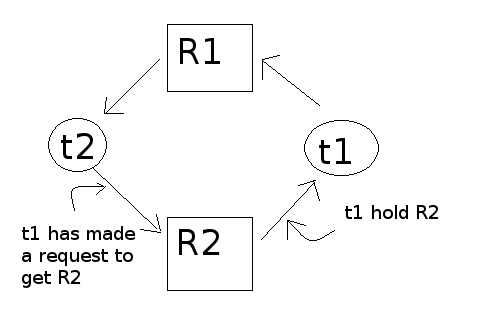
\includegraphics[scale =0.6]{resource_allocation_graph.png}
    \caption{Resource allocation graph}
  \end{center}
\end{figure}

There is a circular wait in the system if there is a cycle in this graph.
$=>$ Detecting a deadlock is easy using this graph ( using, for instance, a bellman-ford algorithm).

Another way to use this graph is to perform a cycle detection for each new request and to decide to refuse it if this induces a cycle in the graph.
This model is not suited if resources are divided into types and if threads ask for one instance of a given resource.
It can be extended :

\begin{figure}[h]
  \begin{center}
    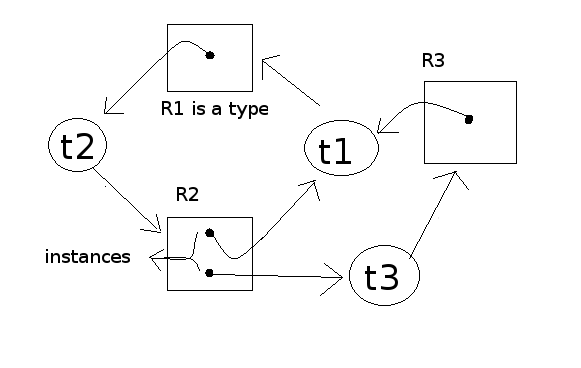
\includegraphics[scale=0.6]{resource_graph_extended}
    \caption{Extended resource allocation graph}
  \end{center}
\end{figure}

In this model, the presence of a cycle doesn't necessarily means that there is a deadlock, only a set of cycles that saturates all the resources it contains, will be a deadlock. $-->$ Not practical.

\section{Allocation matrices and banker algorithm}

At first we assume that we know :

\begin{itemize}
  \item a vector Available such that : Available[i] = number of instances of resources i that are available.
  \item a matrix Allocation such that : Allocation[i][j] = number of resources of type i allocated to thread j.
  \item a matrix Max such that : Max[i][j] = maximal number of resources of type i the thread j will need.
  \item a matrix Need such that : Nedd[i][j] = Max[i][j] - Allocation[i][j]
\end{itemize}

We will try to find if there is an order that make the execution of all threads possible :

\begin{enumerate}
  \item Work = Available
  \item Finished[j] = false for all threads.
  \item while there is some thread j such that : \\ Finished[j] = false \&\& Noeud[i][j] $\leq$ Work[i] $\forall$, \\then : Work[i] += Allocation[i][j] $\forall$ i ; \\Finished[j] =true;
  \item if there is a j such that Finished[j] = false, the system is not in a safe state.
\end{enumerate}

This previous algorithm finds out if the system is in a safe state or not.

For deadlock prevention, we use the banker algorithm : when an allocation request is issue to the system :

\begin{enumerate}

  \item Pretend the request is granted : \\ Available -= request; \\ Allocation[*][j] += request;
  \item run the safe state detection
  \item if the state is not safe, rollback and deny the request.
  
\end{enumerate}

\subsection{Example of the banker algorithm}


  \begin{center}
  Threads
    \begin{tabular}{ccccccc}
       Allocation& A B C & &Available & & Need & A B C\\
       0 & 1 0 1 & & (\textbf{0})1 0 2 & & 0 & 0 2 0 \\
       1 & 0 0 1 & &  & & 1 & 2 1 0\\
       2 & 0 2 0 & &  & & 2 & 0 0 1\\
       3 & (\textbf{2})1 0 0 & &  & & 3 & (\textbf{1})2 2 0\\
       4 & 2 0 0 & &  & & 4 & 2 2 3\\
    \end{tabular}
  \end{center}

Assume that thread 3 requests 1 A resource (1,0,0) (represented in the example with the new numbers between paranthesis)
\begin{enumerate}
  \item Pretend the request is accepted
  \item Run the algorithm to know if the state is safe : Work = (0,0,2). 

  \begin{center}
    \begin{tabular}{cc}
      Thread & Finished\\
      0 & f\\
      1 & f\\
      2 & f\\
      3 & f\\
      4 & f\\
    \end{tabular}
  \end{center}

Thread 2 has needs $\leq$ Work  : Work = (0,2,2).

Thread 0 has needs $\leq$ Work : Work = (1,2,3).

Thread 3 has needs $\leq$ Work : Work = (3,2,3).

Thread 4 has needs $\leq$ Work : Work = (5,2,3).

Thread 1 has needs $\leq$ Work : Work = (5,2,4).

So now we get :

\begin{center}
    \begin{tabular}{cc}
      Thread & Finished\\
      0 & t\\
      1 & t\\
      2 & t\\
      3 & t\\
      4 & t\\
    \end{tabular}
  \end{center}

\item Finished is filled with "true" $=>$ the request can be granted.
\end{enumerate}


\end{document}
